\begin{center}
    \captionof{figure}{Within- and Between-Person Effects of Continuous Predictor and Outcome}

    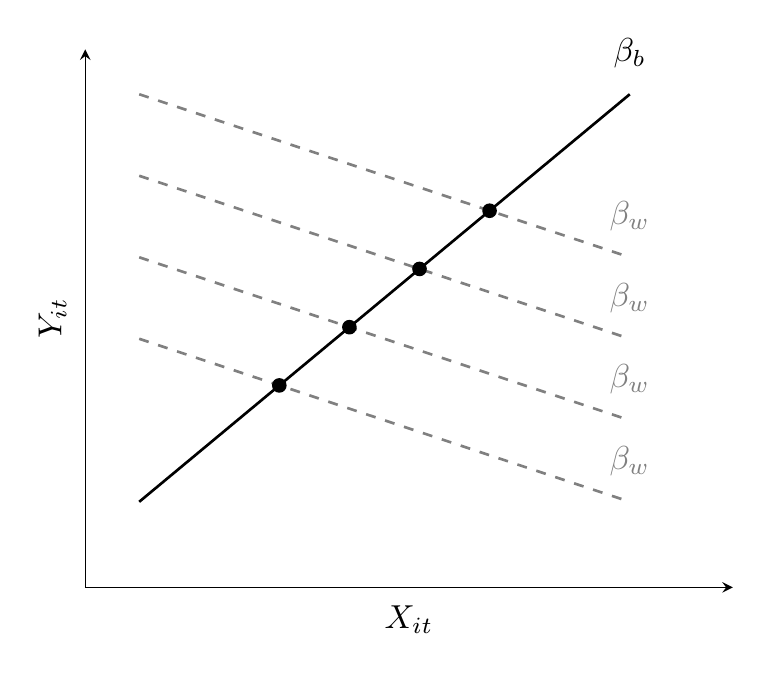
\begin{tikzpicture}[scale=1.2]
        \begin{axis}[
            axis x line=left, 
            axis y line=left, 
            xlabel={$X_{it}$}, ylabel={$Y_{it}$},
            xmin=0, xmax=1.1, ymin=0, ymax=1.1,
            xtick=\empty, % Tick at 0 and 1
            ytick=\empty,
            enlargelimits=true,
            clip=false,
            xshift=-15mm  % Shift Y-axis further left
        ]
    
        % Define parameters
        \pgfmathsetmacro{\intercept}{0.1}  % Intercept of the between-person line
        \pgfmathsetmacro{\slopeB}{1}     % Slope for Beta_B
        \pgfmathsetmacro{\slopeW}{-0.4}    % Slope for Beta_W
    
        % Main regression line (Between-Person Effect)
        \addplot[black, thick] expression[domain=0:1, samples=2] {\intercept + \slopeB * x};
        \node[black] at (axis cs: 1, 1.2) {$\beta_\text{b}$}; % Label for Beta_B
    
        % Parallel within-group lines (Within-Person Effect)
        \foreach \shift in {0.2, 0.4, 0.6, 0.8} {
            \addplot[gray, thick, dashed] expression[domain=0:1, samples=2] {1.3 - \shift + \slopeW * x};
    
            % Compute X-value at intersection with the between-person line:
            \pgfmathsetmacro{\xintersect}{(\shift +0.1 + \intercept) / (\slopeB - \slopeW)}
            \pgfmathsetmacro{\yintersect}{\intercept + \slopeB * \xintersect}
    
            % Add dot at intersection
            \addplot[black, only marks, mark=*] coordinates {(\xintersect, \yintersect)};
    
        }
    
        % Labels for within-group slopes
        \node[gray] at (axis cs: 1, 0.8) {$\beta_\text{w}$};
        \node[gray] at (axis cs: 1, 0.6) {$\beta_\text{w}$};
        \node[gray] at (axis cs: 1, 0.4) {$\beta_\text{w}$};
        \node[gray] at (axis cs: 1, 0.2) {$\beta_\text{w}$};
    
    \end{axis}
    \end{tikzpicture}

    \label{fig:withinbetween-contxy}
    \begin{figurenote}
        The solid black slope represents the between-person effect and the dashed solid grey slopes the within-cluster effect. The X-axis simultaneously represents $X_{it}$ for the within-slope and $\mu_{X,i}$ for the between-slope.
    \end{figurenote}
\end{center}